\documentclass[10pt,aspectratio=43]{beamer}

\usepackage{graphicx}
\usepackage{tikz}
\usepackage{xcolor}
\usepackage{caption}
\usepackage{subcaption}
\usepackage{bm}
\usetikzlibrary{calc} 
\usepackage{hyperref}
\hypersetup{
    colorlinks=true,
    linkcolor=blue,
    urlcolor=red
}
\usepackage{fontawesome5}
\usepackage{ulem}

\usetheme{MyStyle}   % loads beamerthemeMyStyle.sty
\setlength{\columnsep}{0pt}


%%%%%%%%%%%%%%%%%%%%%%%%%%%%%%%%%%%%%%%%%%
%%%%%%%%%%%%%%%%%%%%%%%%%%%%%%%%%%%%%%%%%%
%%%%%%%%%%%%%%%%%%%%%%%%%%%%%%%%%%%%%%%%%%

\title{Layer alignment}
\newcommand{\eventname}{ALERT meeting}
\author{Felix Touchte Codjo}
\institute{IJCLab}
\date{\today}


\begin{document}

\begin{frame}[plain] % remove header, footer, barre de navigation
\titlepage
\end{frame}

%\begin{frame}{Outline}
%\tableofcontents
%\end{frame}

%\section{Intro}
\section{Updates}

\begin{frame}{Layer alignment}
    \begin{itemize}
        \item Before alignment
    \end{itemize}

    \centering
    \vspace{0.2cm}

    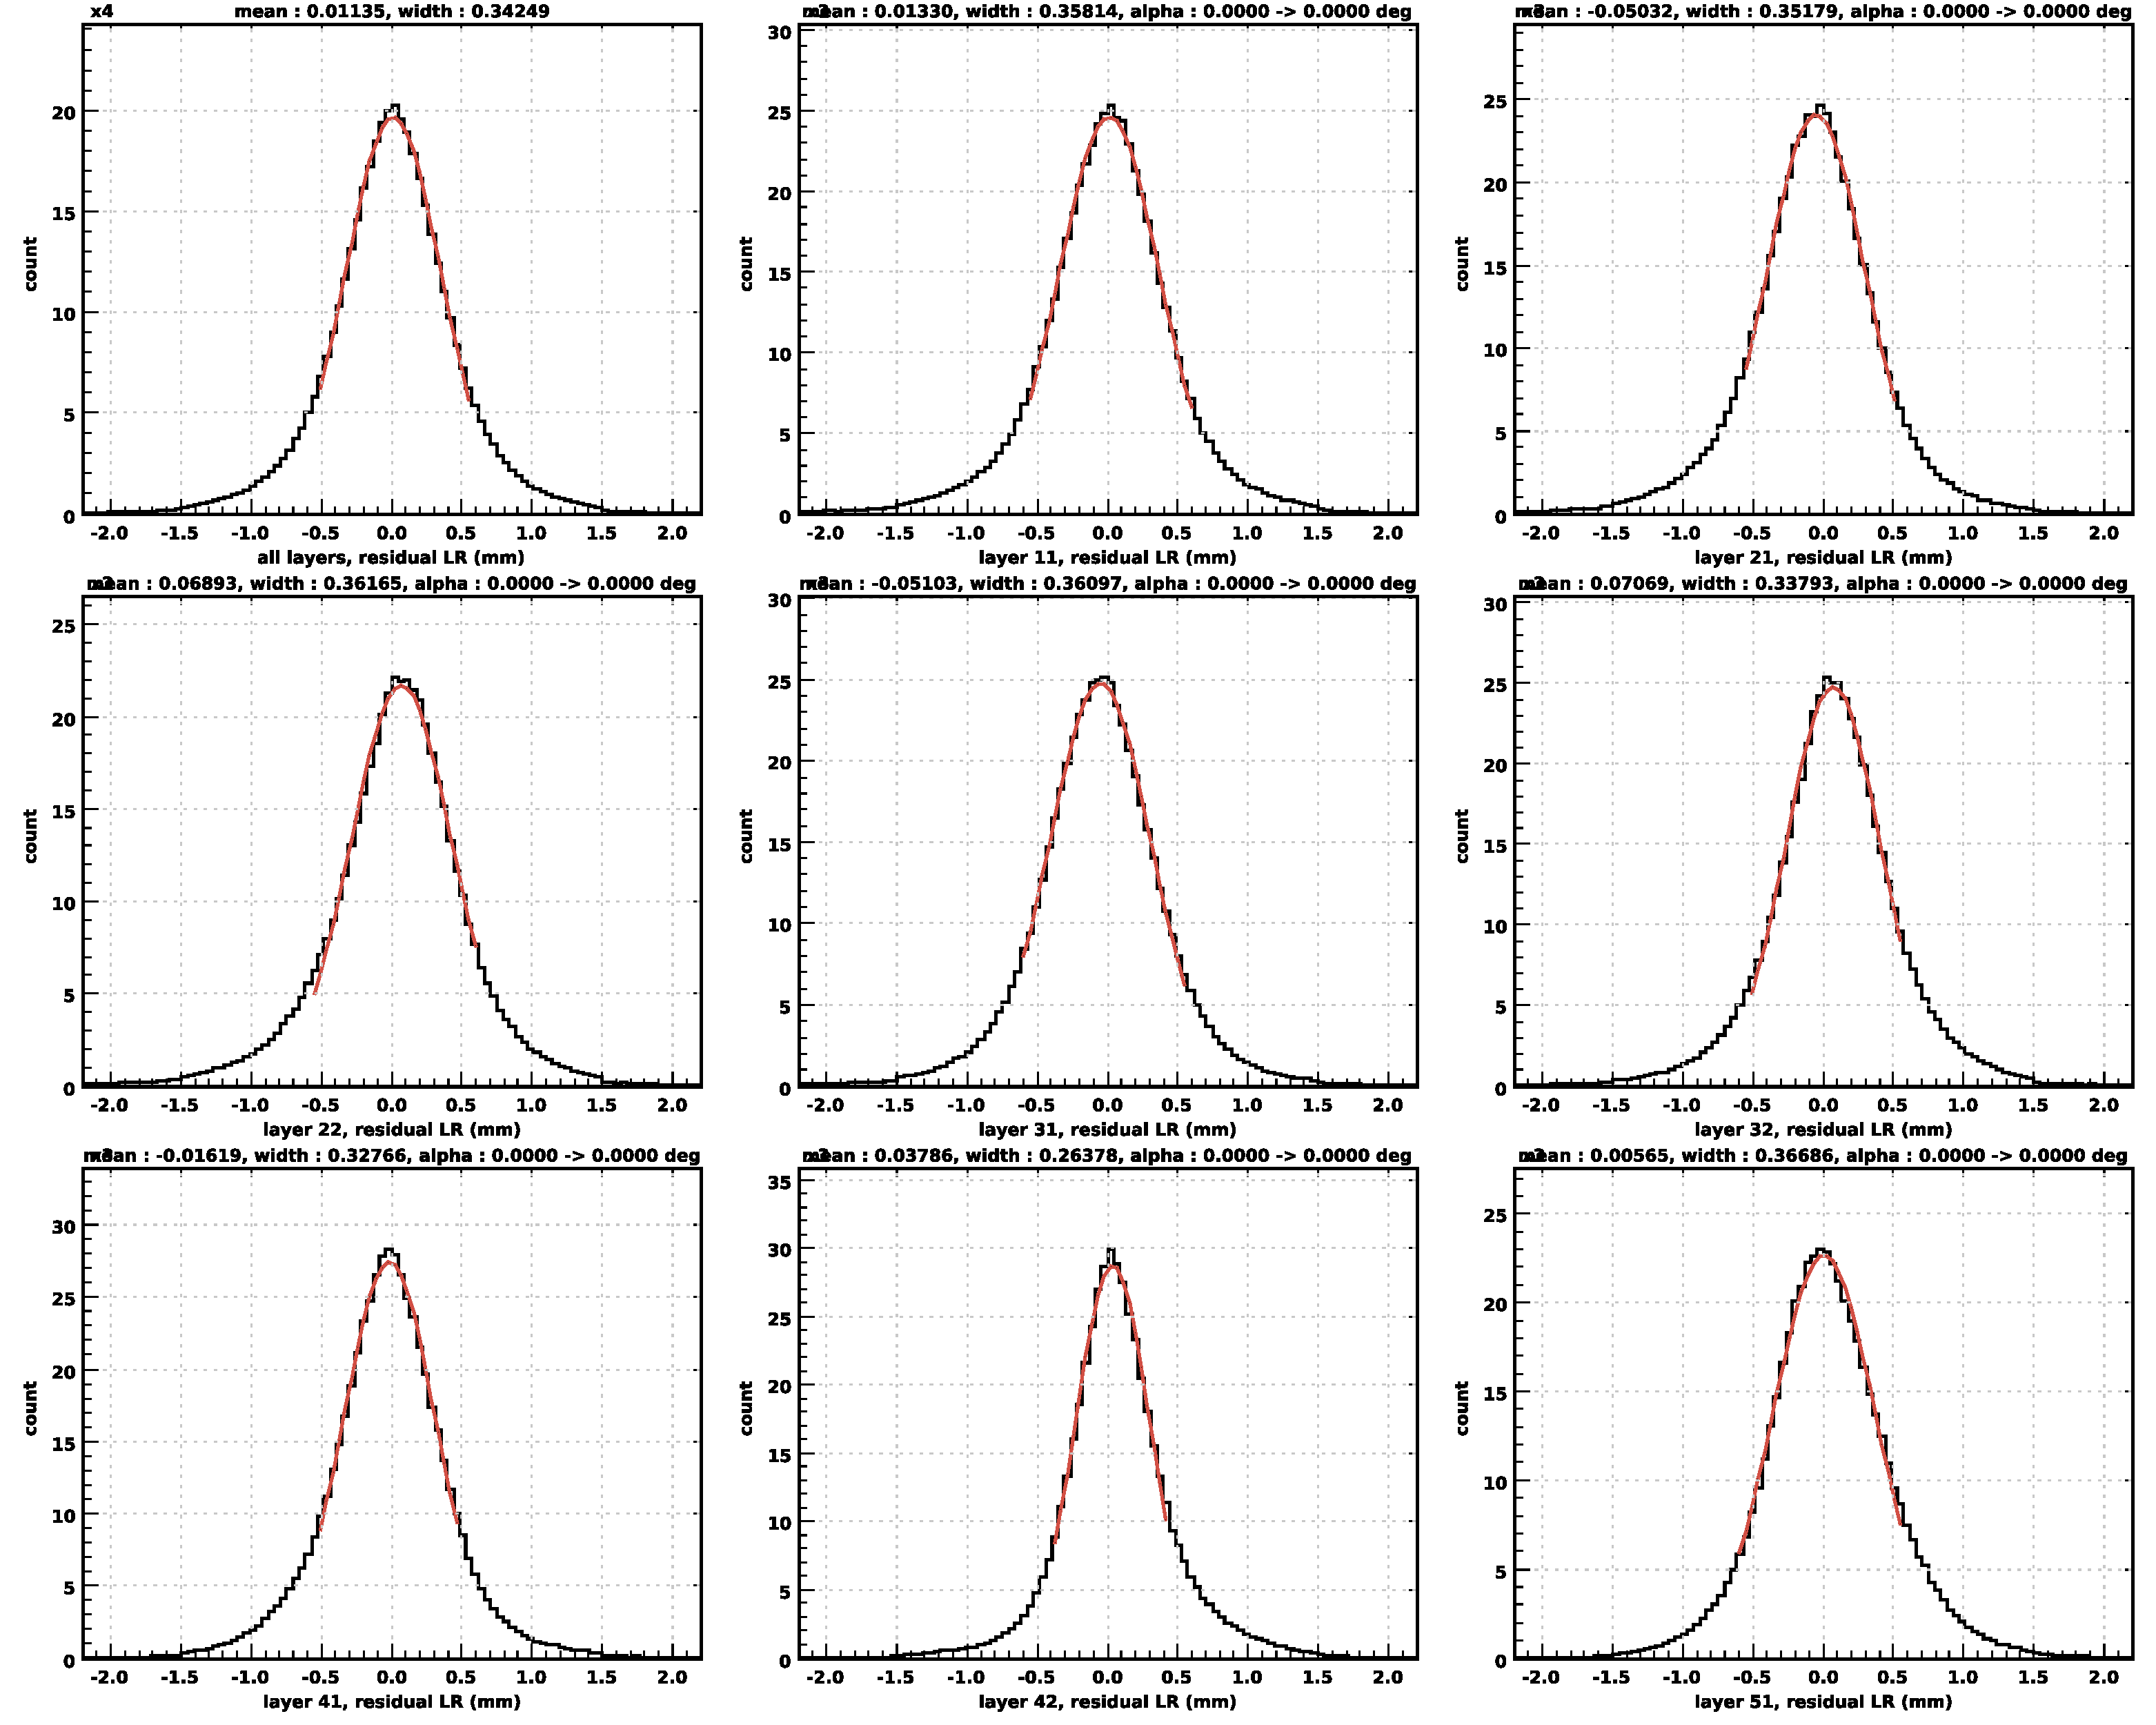
\includegraphics[width=0.7\linewidth]{figures/residual_LR_iter_1_before.pdf}
\end{frame}

\begin{frame}{Layer alignment}
    \begin{itemize}
        \item After alignment
    \end{itemize}

    \centering
    \vspace{0.2cm}

    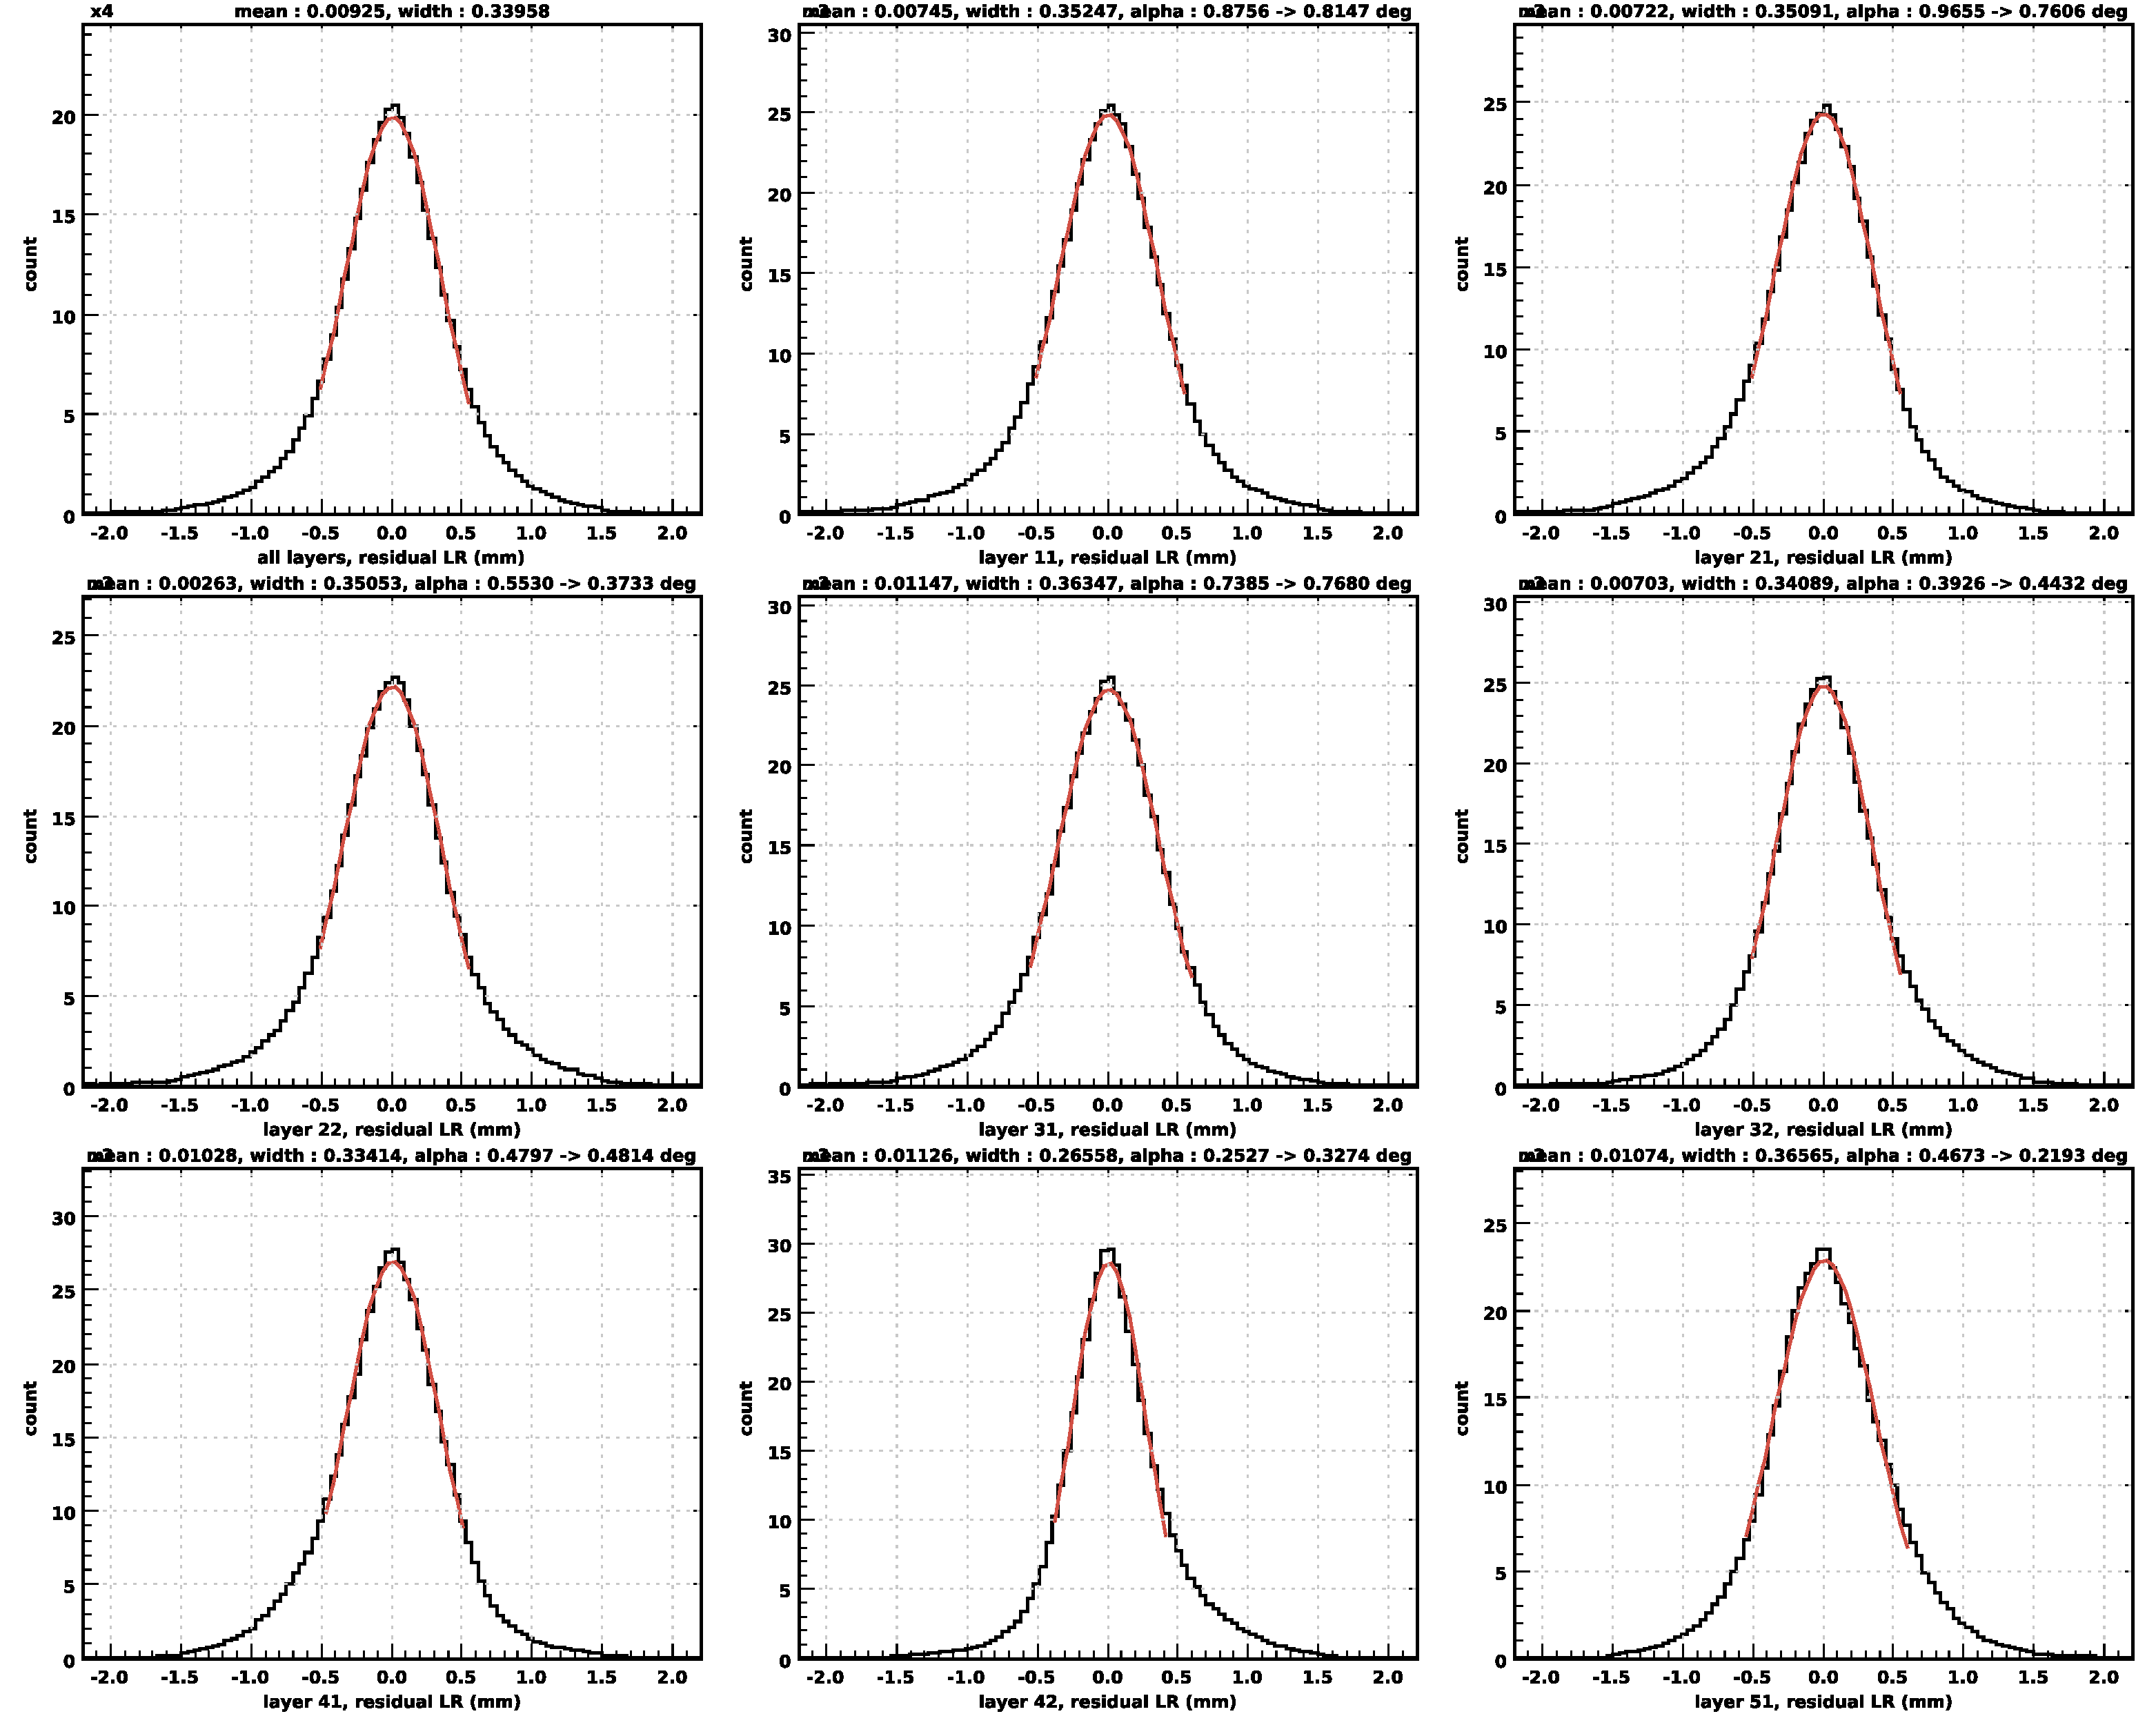
\includegraphics[width=0.7\linewidth]{figures/residual_LR_iter_1_after.pdf}
\end{frame}


\begin{frame}{Layer alignment}
    \begin{itemize}
        \item Before alignment
    \end{itemize}

    \centering
    \vspace{0.2cm}

    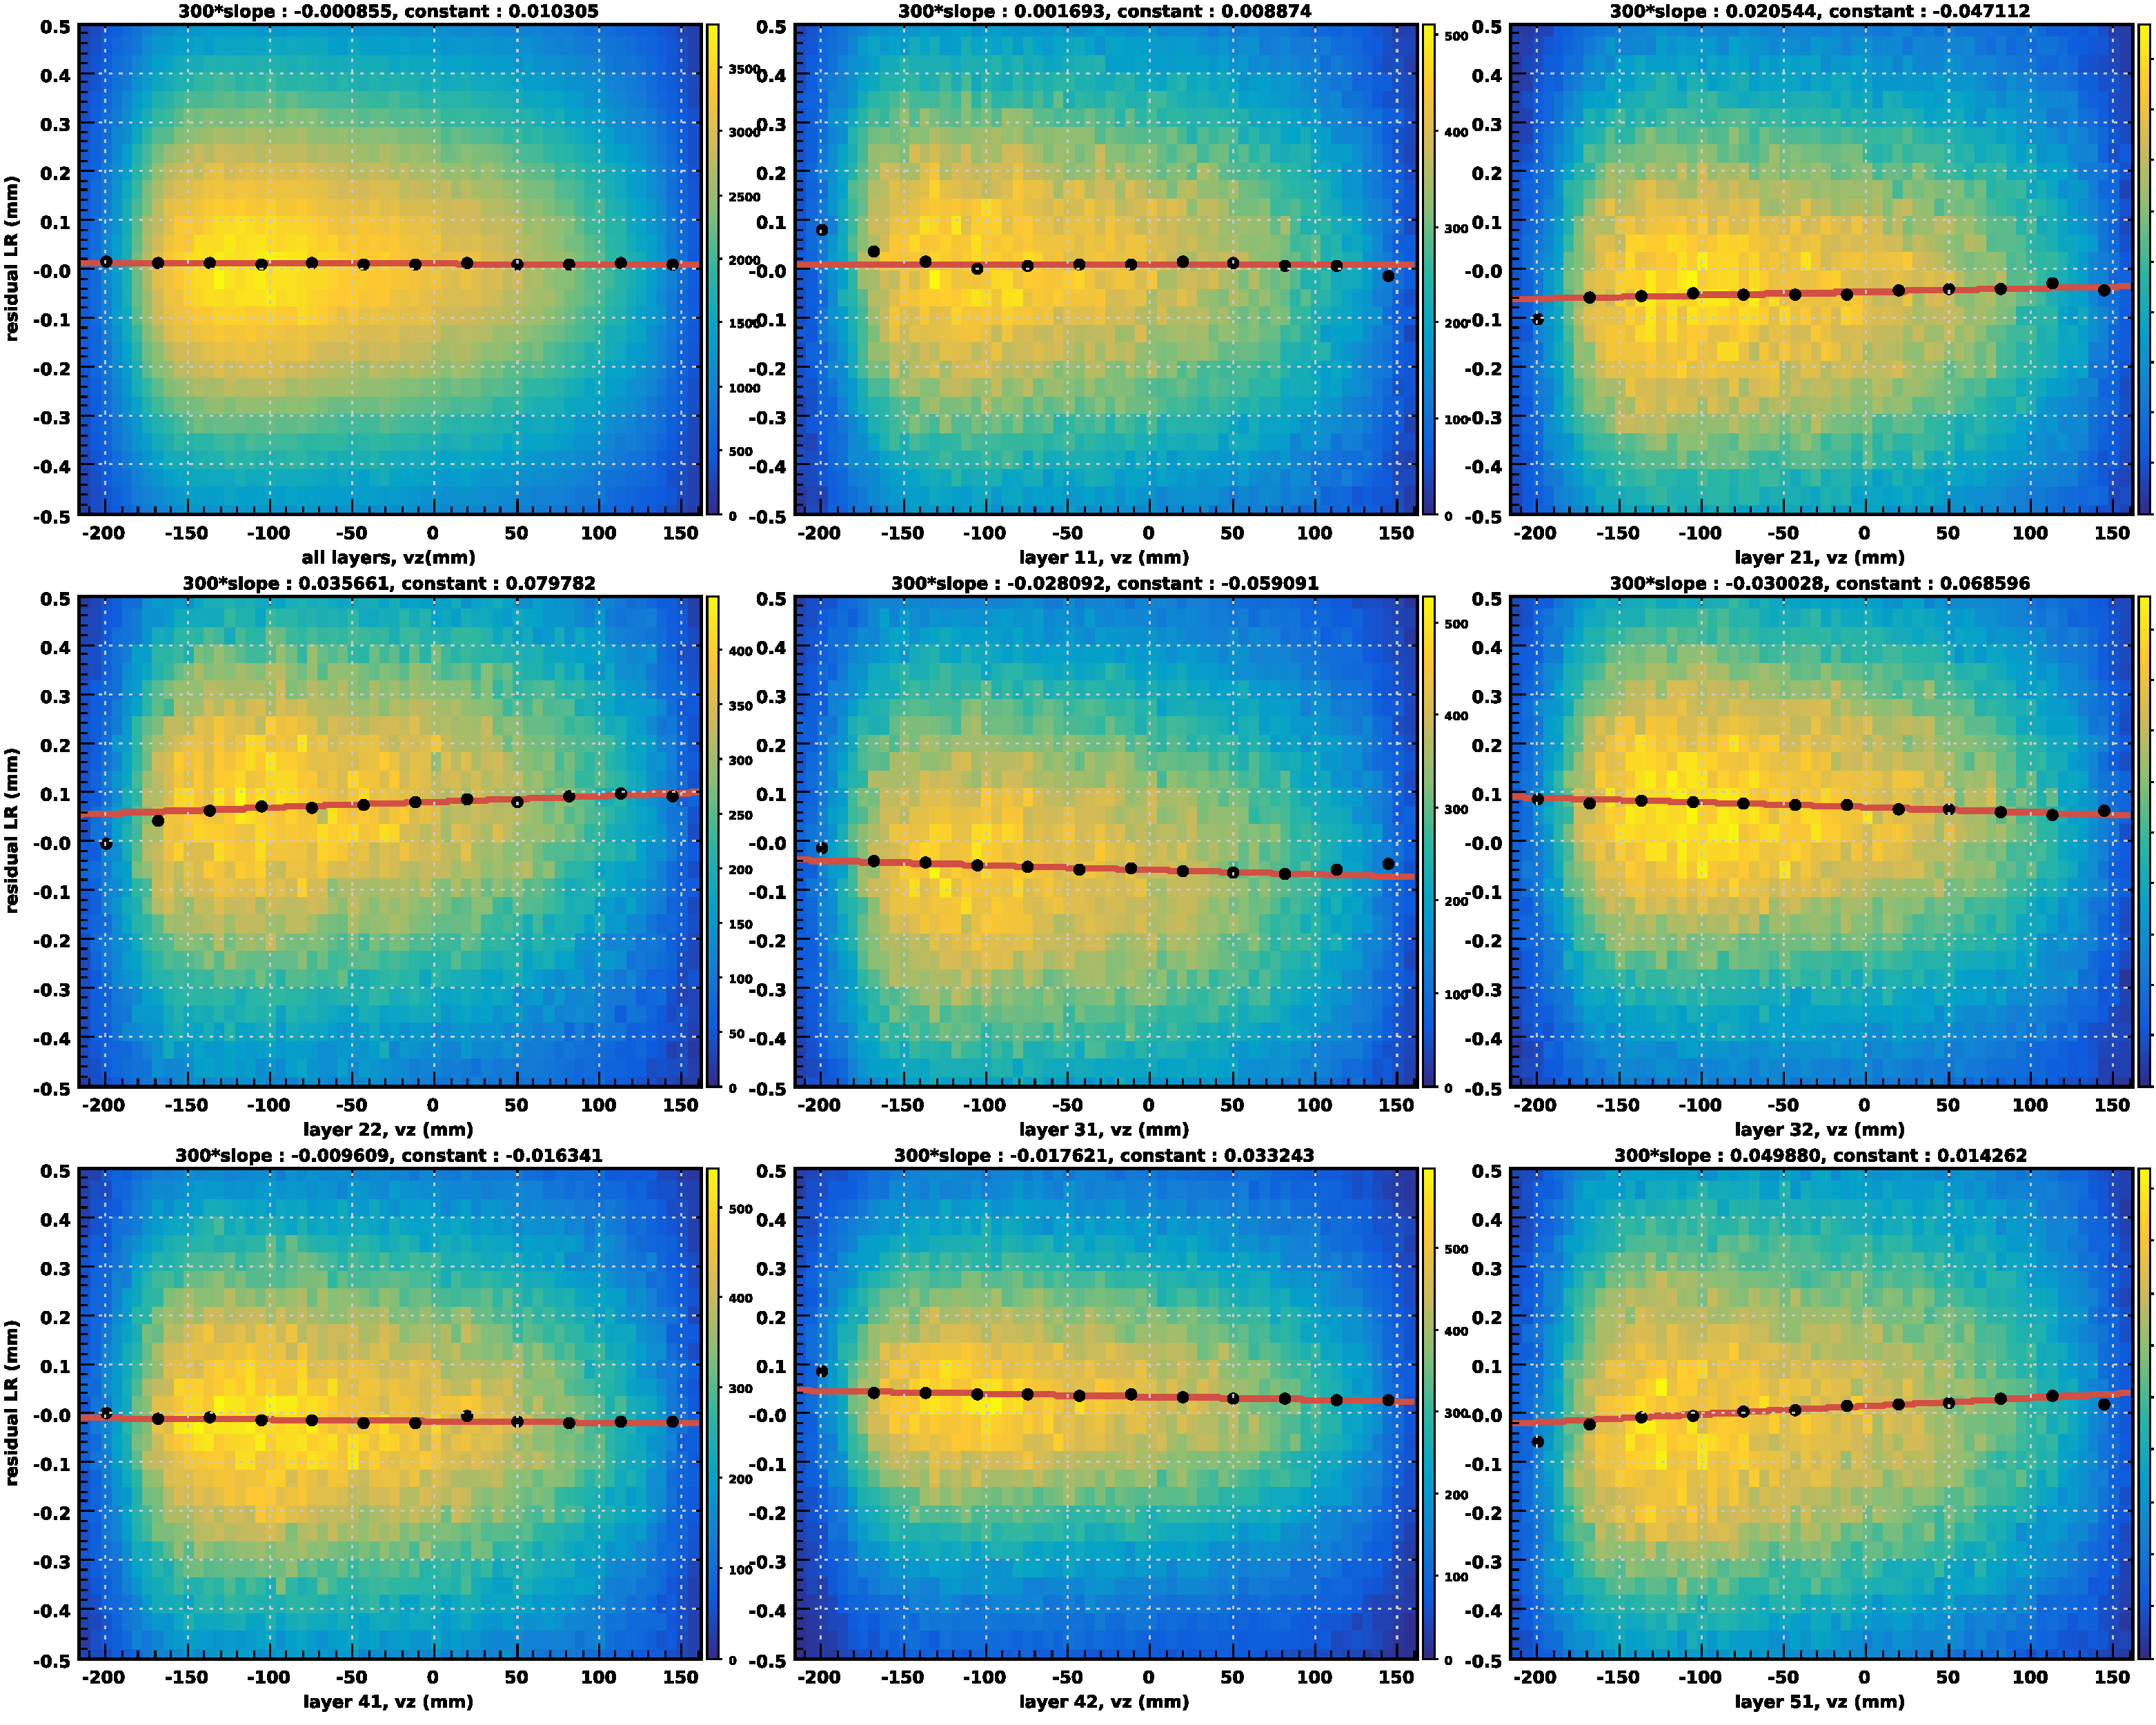
\includegraphics[width=0.7\linewidth]{figures/corr_vz_residual_LR_iter_1_before.pdf}
\end{frame}

\begin{frame}{Layer alignment}
    \begin{itemize}
        \item After alignment
    \end{itemize}

    \centering
    \vspace{0.2cm}

    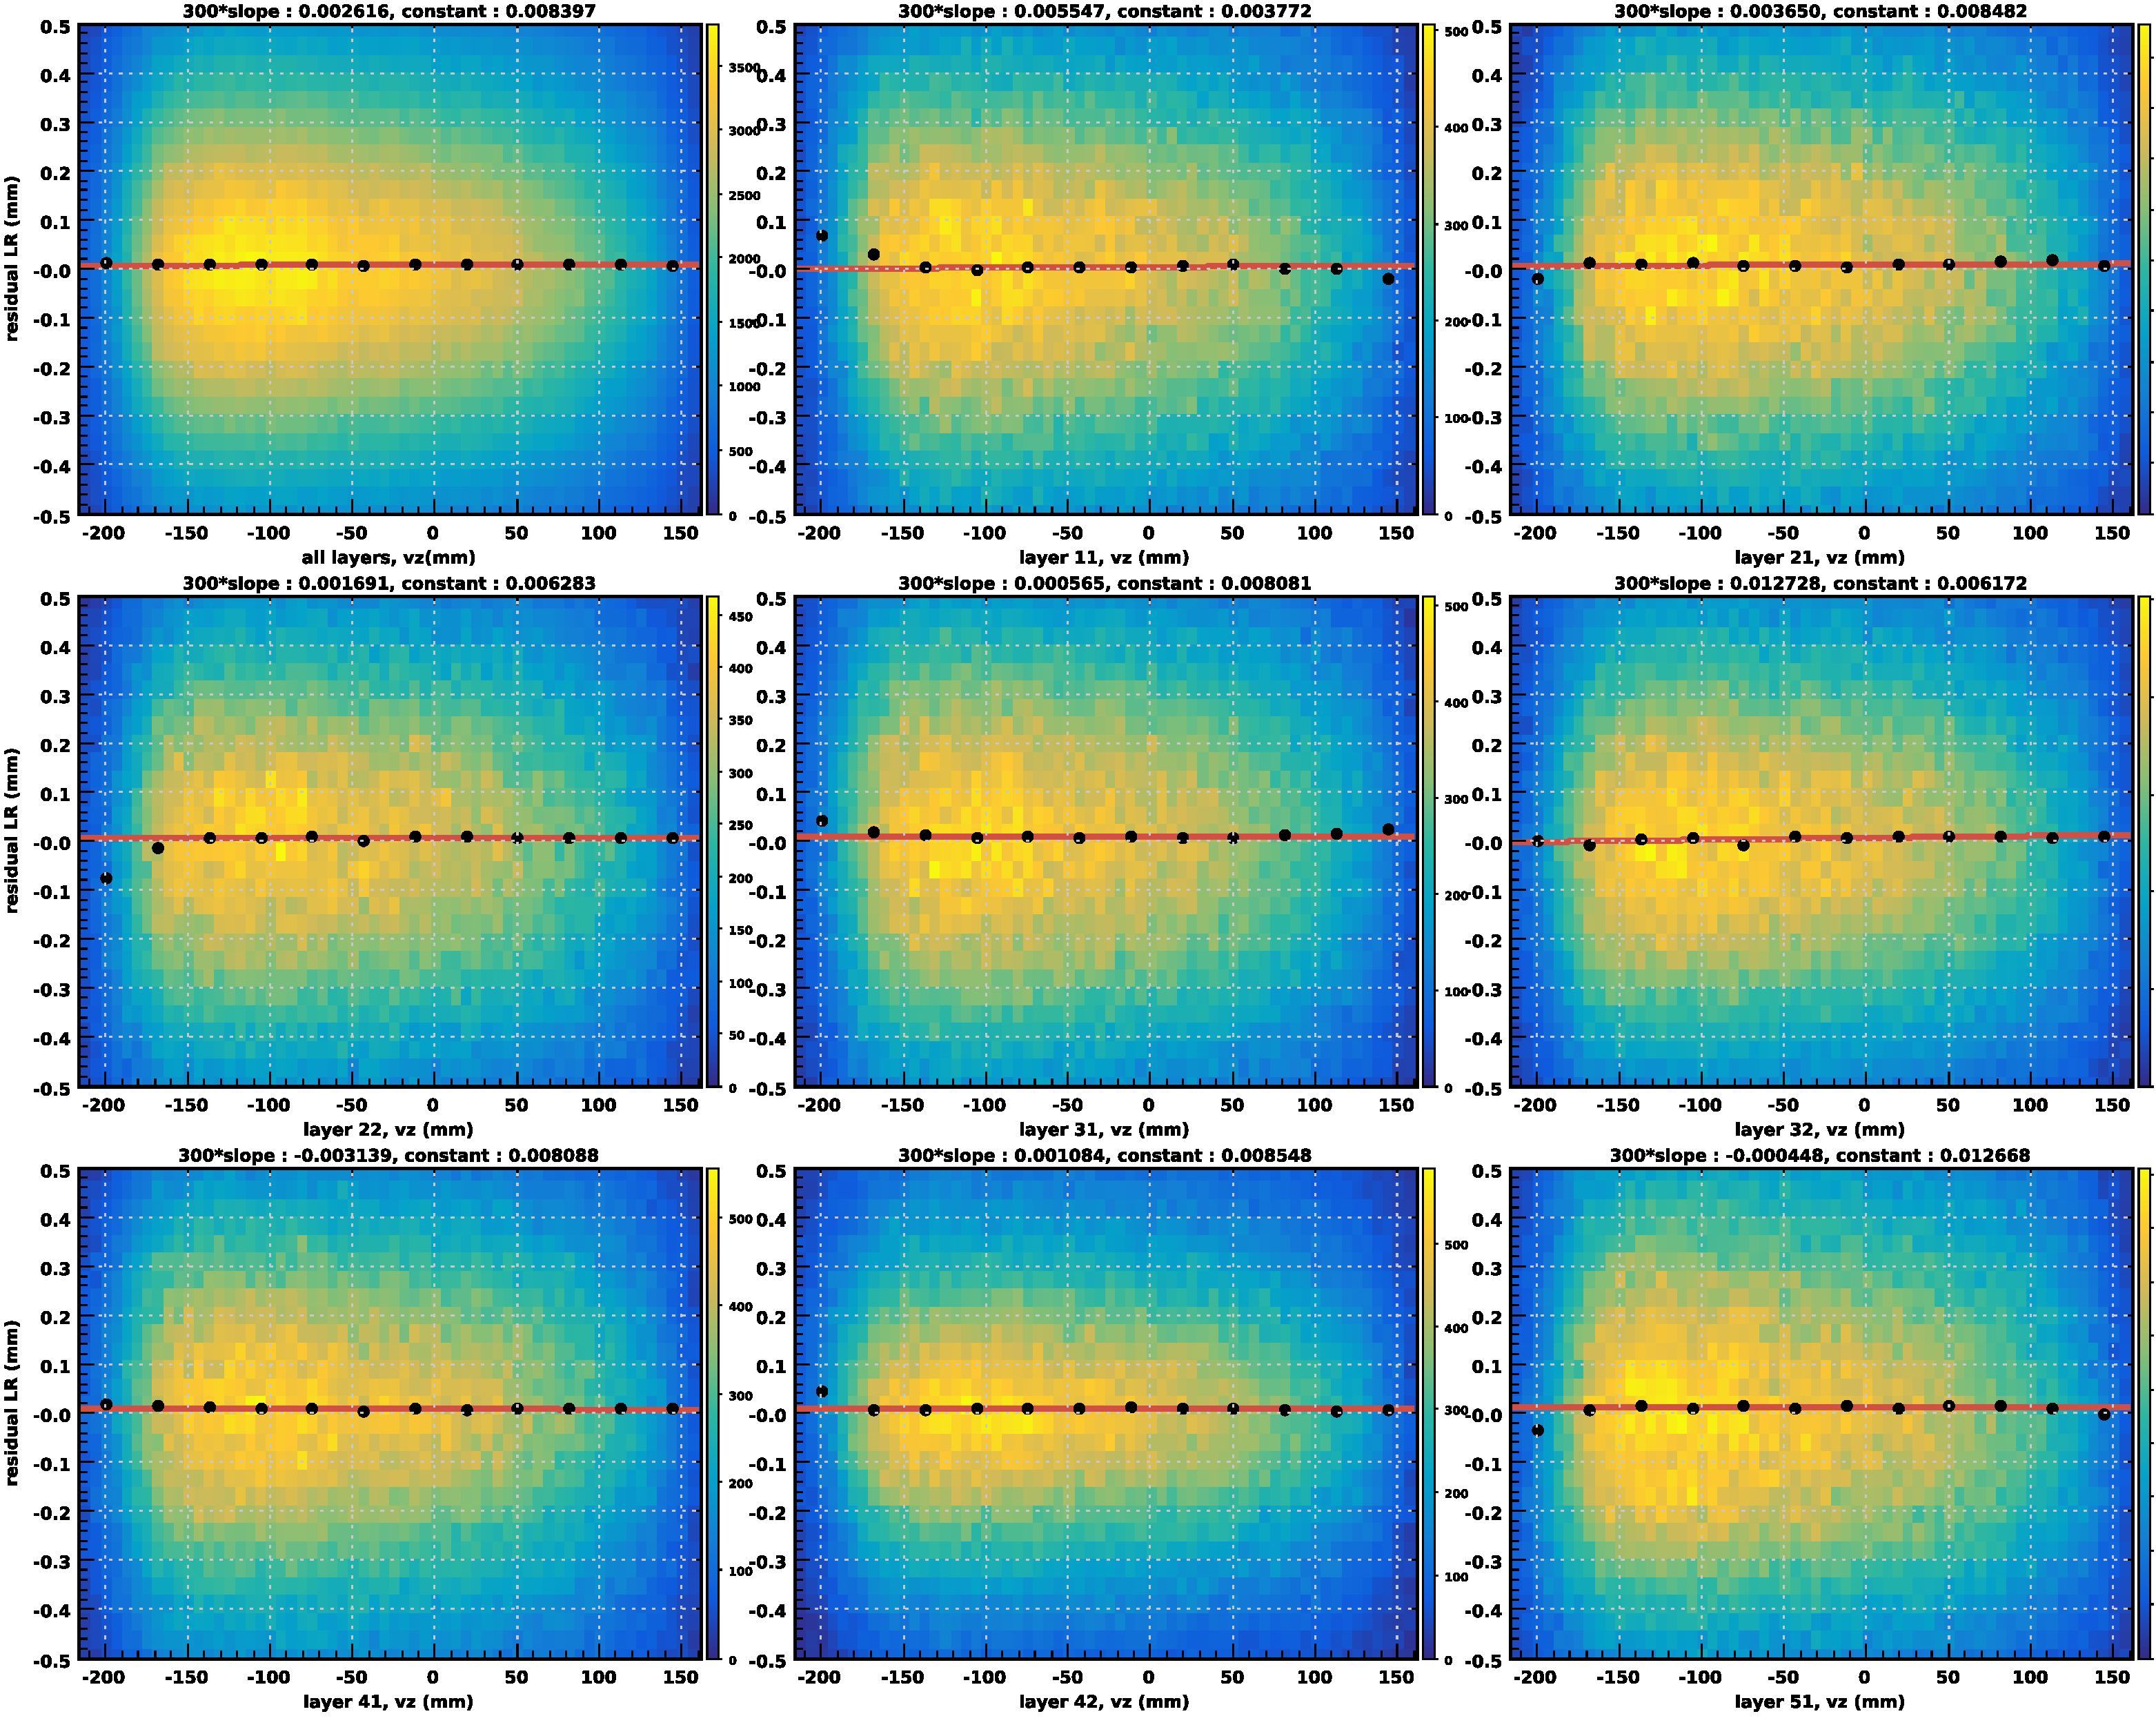
\includegraphics[width=0.7\linewidth]{figures/corr_vz_residual_LR_iter_1_after.pdf}
\end{frame}

\begin{frame}{Layer alignment}
    \begin{itemize}
        \item Time2distance after alignment : probably the main limitation
    \end{itemize}

    \centering
    \vspace{0.2cm}

    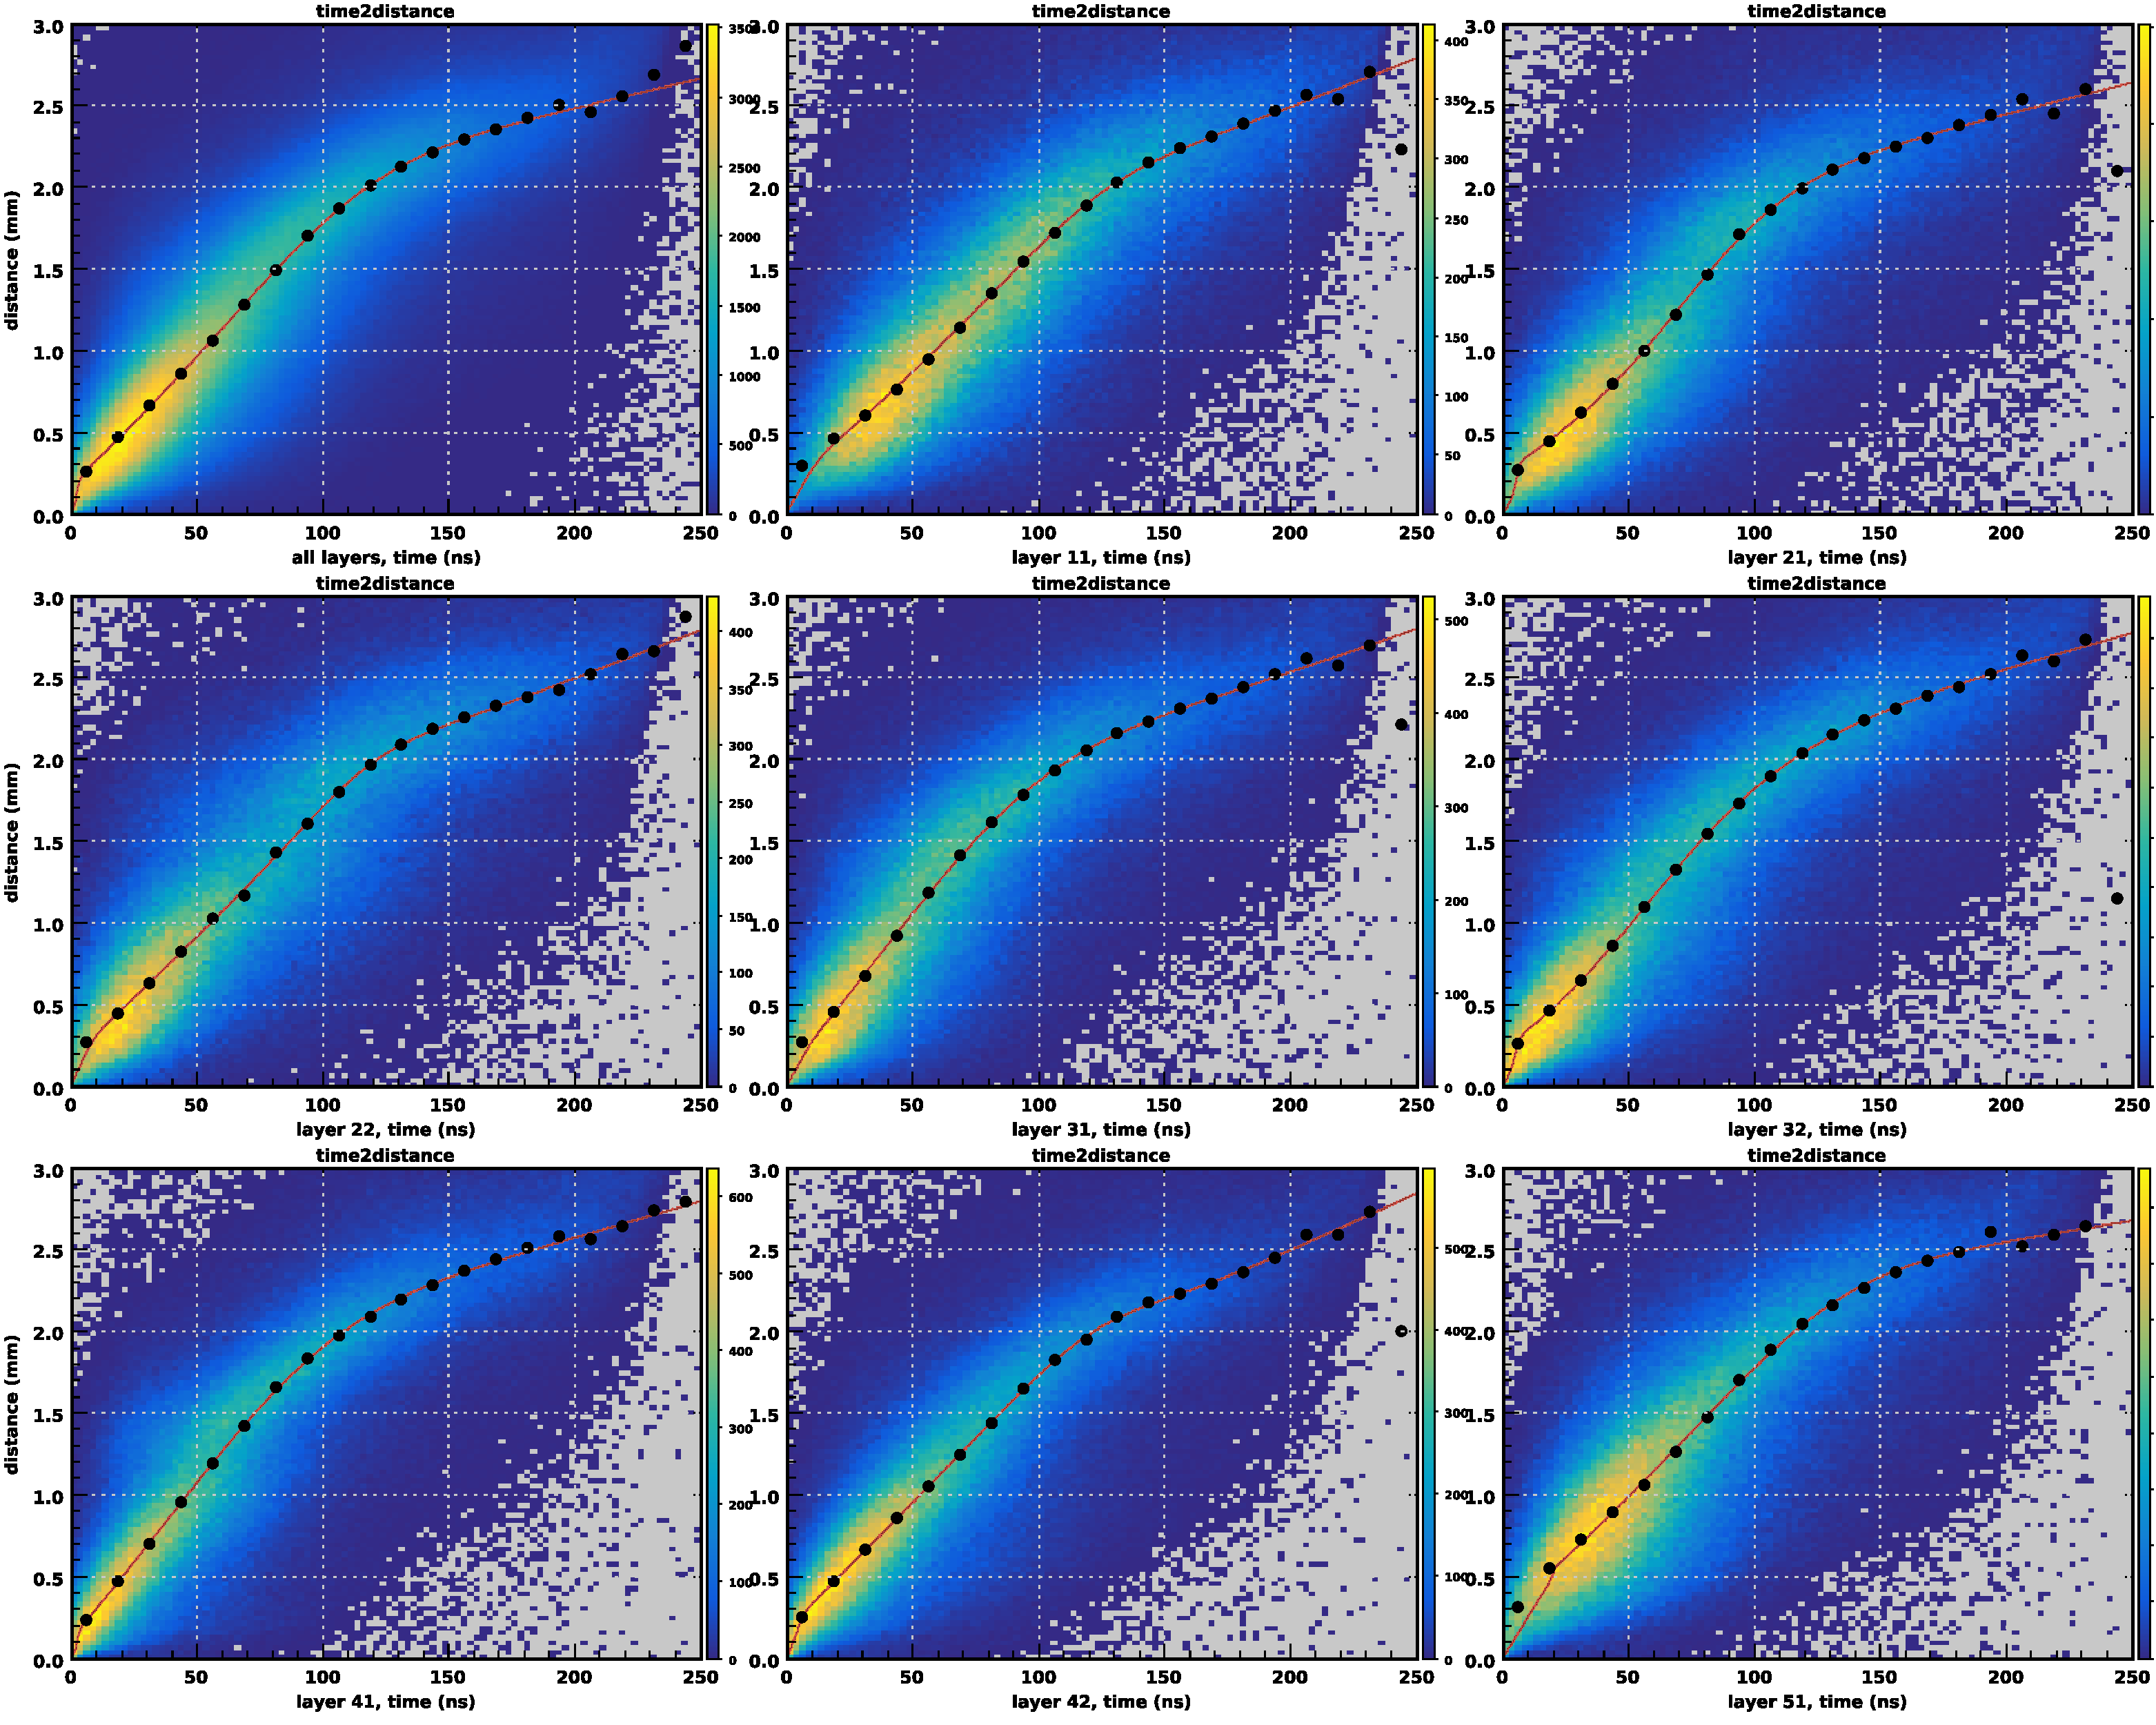
\includegraphics[width=0.7\linewidth]{figures/time2distance_iter_1_after_as_limitation.pdf}
\end{frame}





\end{document}


